\section{Problématique}
Nous voudrions construire un système dans lequel il existe plusieurs vendeurs et plusieurs centres de ventes. Chaque vendeur propose ses produits en ligne, les centres de ventes à leur tour après avoir reçu une requête d’un acheteur, contactent les vendeurs suspectés d’avoir le produit recherché et retourne le résultat à l’utilisateur. Par exemple: 
On peut avoir les centres suivants:
\begin{itemize}
\item Centre de vente d’appareil électronique.
\item Centre de vente de vêtements.
\end{itemize}
Les vendeurs:
\begin{itemize}
\item Vendeur de chaussures.
\item Vendeur de téléphone portable.
\item Vendeur de pantalon.
\item Vendeur d’ordinateur.
\end{itemize}

On remarque que les centres sont caractérisés par une catégorie générale tandis que les vendeurs sont typiquement plus spécialisé dans un domaine donné, l’avantage de cette méthode est que l’utilisateur ne se soucie pas de la recherche du vendeur qui possède le produit recherché. Il va directement poser sa requête auprès d’un centre de ventes, et c’est à ce dernier de chercher le produit chez les vendeurs. Dans l’exemple précédent si le centre de vente d’appareil électronique reçoit une requête recherchant un ordinateur portable avec des paramètres donnés. Il va directement contacté le ou les vendeurs susceptible d’avoir le produit recherché, et donc le vendeur d’ordinateur.


Les vendeurs eux aussi n’ont pas à s’enregistrer chez les centres de ventes. Ils seront intelligemment contactés par ces derniers lors du traitement d’une requête donnée.\\

Pour réaliser un tel système de ventes nous allons nous baser sur un système multi-agents pour gérer la communication entre les centres de ventes et les vendeurs, ainsi que le traitement intelligent des requêtes utilisateurs.
\newpage
\section{Définitions}
\subsection{Agent intelligent}
Un agent est un logiciel qui agit de façon autonome. C'est un programme qui accomplit des tâches à la manière d'un automate et en fonction de ce que lui a demandé son auteur, en revanche un \textbf{agent intelligent} est une entité autonome capable de percevoir son environnement grâce à des capteurs et aussi d'agir sur celui-ci via des effecteurs afin de réaliser des buts1. Un agent intelligent peut également apprendre ou utiliser des connaissances pour pouvoir réaliser ses objectifs.
\begin{figure}[H]
	\centering
	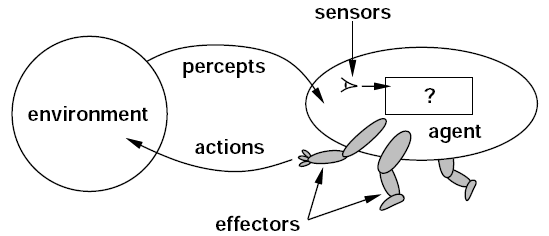
\includegraphics[width=0.5\textwidth]{imgs/intelligentAgent.png}
	\caption{Agent intelligent interagissant avec le monde extérieur }
\end{figure}

\subsection{Système multi-agents}
un système multi-agents (SMA) est un système composé d'un ensemble d'agents (un processus, un robot, un être humain, etc.), situés dans un certain environnement et interagissant selon certaines relations. Un agent est une entité caractérisée par le fait qu'elle est, au moins partiellement, autonome.
\begin{figure}[H]
	\centering
	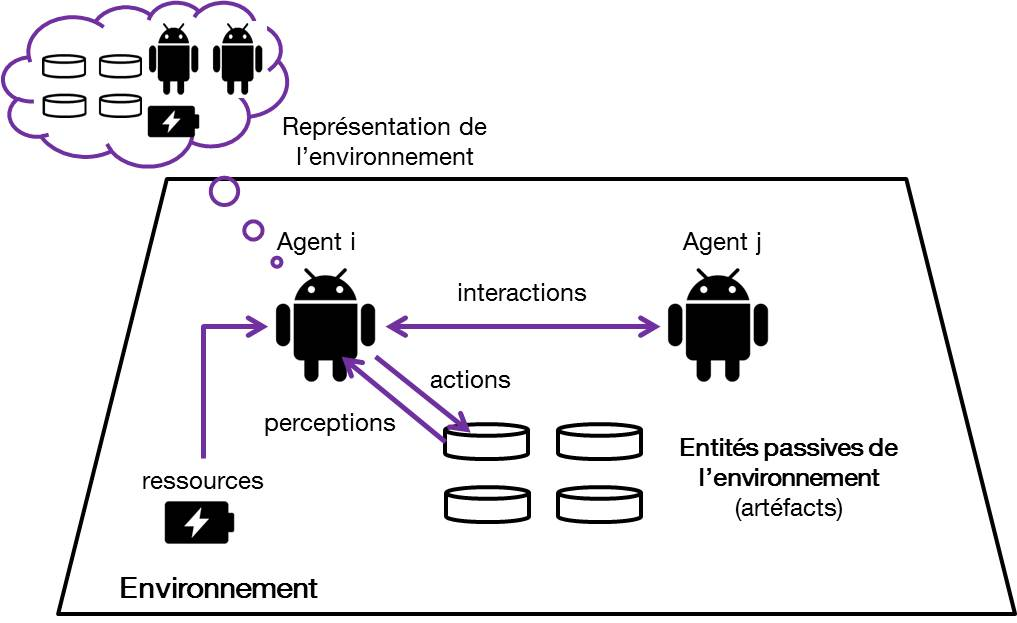
\includegraphics[width=0.5\textwidth]{imgs/SMA.jpg}
	\caption{Système multi-agents en coopération}
\end{figure}

